% Generated by hgg-latex
\documentclass[border=0pt]{standalone}
\usepackage[T1]{fontenc}
\usepackage{DejaVuSans}
\usepackage{tikz}
\definecolor{pcFFFFFF}{HTML}{FFFFFF}
\definecolor{pcDDDDDD}{HTML}{DDDDDD}
\definecolor{pc444444}{HTML}{444444}
\definecolor{pc333333}{HTML}{333333}
\definecolor{pc1F77B4}{HTML}{1F77B4}
\begin{document}
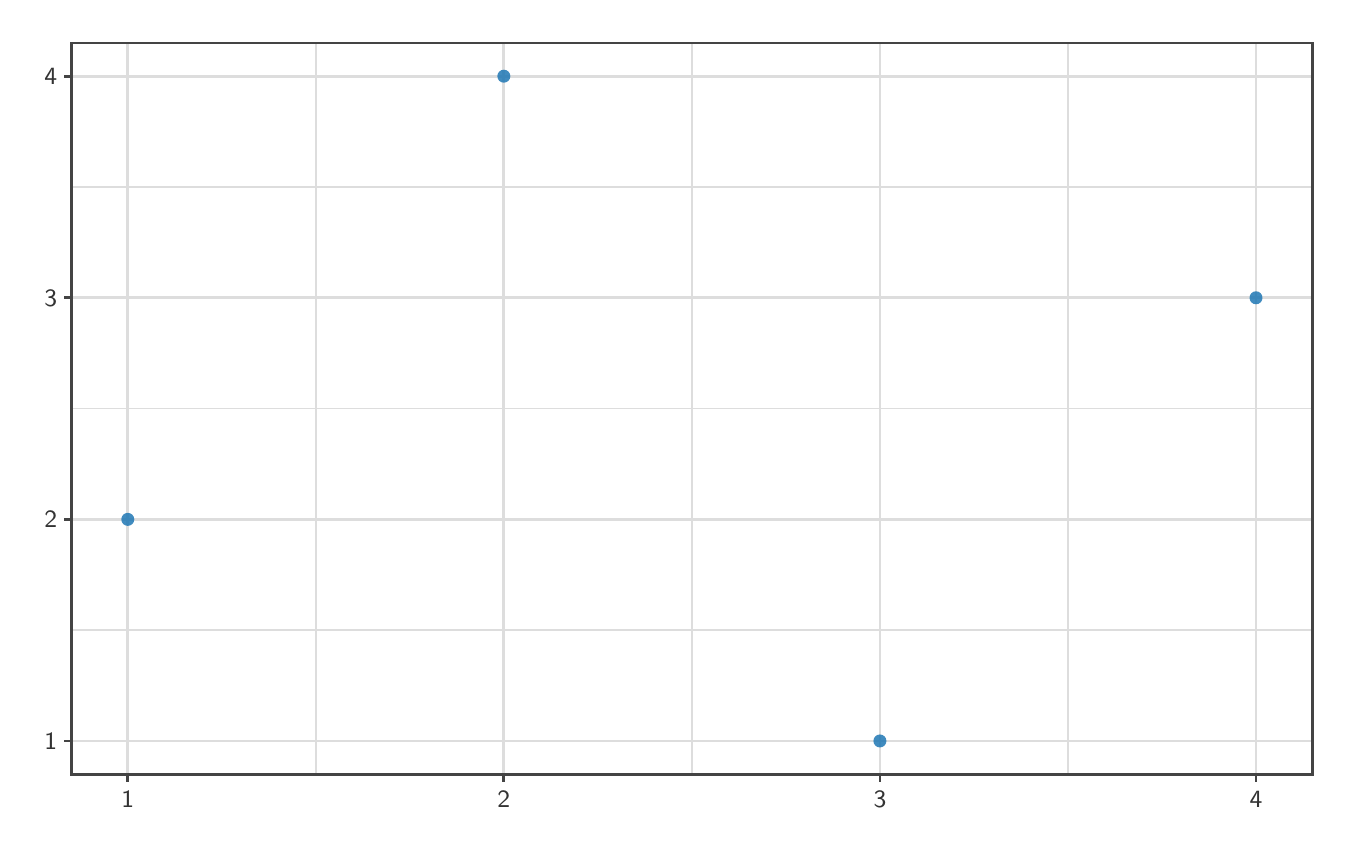
\begin{tikzpicture}
\path[use as bounding box] (0bp,0bp) rectangle (468.000bp,288.000bp);
\path[fill=pcFFFFFF] (0.000bp,0.000bp) rectangle (468.000bp,288.000bp);
\draw[line width=0.500bp, color=pcDDDDDD] (103.730bp,282.500bp) -- (103.730bp,19.250bp);
\draw[line width=0.500bp, color=pcDDDDDD] (239.115bp,282.500bp) -- (239.115bp,19.250bp);
\draw[line width=0.500bp, color=pcDDDDDD] (374.500bp,282.500bp) -- (374.500bp,19.250bp);
\draw[line width=1.000bp, color=pcDDDDDD] (36.038bp,282.500bp) -- (36.038bp,19.250bp);
\draw[line width=1.000bp, color=pcDDDDDD] (171.423bp,282.500bp) -- (171.423bp,19.250bp);
\draw[line width=1.000bp, color=pcDDDDDD] (306.807bp,282.500bp) -- (306.807bp,19.250bp);
\draw[line width=1.000bp, color=pcDDDDDD] (442.192bp,282.500bp) -- (442.192bp,19.250bp);
\draw[line width=0.500bp, color=pcDDDDDD] (15.730bp,71.102bp) -- (462.500bp,71.102bp);
\draw[line width=0.500bp, color=pcDDDDDD] (15.730bp,150.875bp) -- (462.500bp,150.875bp);
\draw[line width=0.500bp, color=pcDDDDDD] (15.730bp,230.648bp) -- (462.500bp,230.648bp);
\draw[line width=1.000bp, color=pcDDDDDD] (15.730bp,31.216bp) -- (462.500bp,31.216bp);
\draw[line width=1.000bp, color=pcDDDDDD] (15.730bp,110.989bp) -- (462.500bp,110.989bp);
\draw[line width=1.000bp, color=pcDDDDDD] (15.730bp,190.761bp) -- (462.500bp,190.761bp);
\draw[line width=1.000bp, color=pcDDDDDD] (15.730bp,270.534bp) -- (462.500bp,270.534bp);
\path[fill=pcFFFFFF, fill opacity=0.000, draw=pc444444, line width=1.000bp] (15.730bp,19.250bp) rectangle (462.500bp,282.500bp);
\draw[line width=1.000bp, color=pc444444] (36.038bp,19.250bp) -- (36.038bp,16.500bp);
\node[anchor=base, inner sep=0, text=pc333333] at (36.038bp,7.260bp) {\sffamily\fontsize{8.800bp}{10.560bp}\selectfont 1};
\draw[line width=1.000bp, color=pc444444] (171.423bp,19.250bp) -- (171.423bp,16.500bp);
\node[anchor=base, inner sep=0, text=pc333333] at (171.423bp,7.260bp) {\sffamily\fontsize{8.800bp}{10.560bp}\selectfont 2};
\draw[line width=1.000bp, color=pc444444] (306.807bp,19.250bp) -- (306.807bp,16.500bp);
\node[anchor=base, inner sep=0, text=pc333333] at (306.807bp,7.260bp) {\sffamily\fontsize{8.800bp}{10.560bp}\selectfont 3};
\draw[line width=1.000bp, color=pc444444] (442.192bp,19.250bp) -- (442.192bp,16.500bp);
\node[anchor=base, inner sep=0, text=pc333333] at (442.192bp,7.260bp) {\sffamily\fontsize{8.800bp}{10.560bp}\selectfont 4};
\draw[line width=1.000bp, color=pc444444] (15.730bp,31.216bp) -- (12.980bp,31.216bp);
\node[anchor=base east, inner sep=0, text=pc333333] at (10.780bp,28.136bp) {\sffamily\fontsize{8.800bp}{10.560bp}\selectfont 1};
\draw[line width=1.000bp, color=pc444444] (15.730bp,110.989bp) -- (12.980bp,110.989bp);
\node[anchor=base east, inner sep=0, text=pc333333] at (10.780bp,107.909bp) {\sffamily\fontsize{8.800bp}{10.560bp}\selectfont 2};
\draw[line width=1.000bp, color=pc444444] (15.730bp,190.761bp) -- (12.980bp,190.761bp);
\node[anchor=base east, inner sep=0, text=pc333333] at (10.780bp,187.681bp) {\sffamily\fontsize{8.800bp}{10.560bp}\selectfont 3};
\draw[line width=1.000bp, color=pc444444] (15.730bp,270.534bp) -- (12.980bp,270.534bp);
\node[anchor=base east, inner sep=0, text=pc333333] at (10.780bp,267.454bp) {\sffamily\fontsize{8.800bp}{10.560bp}\selectfont 4};
\path[fill=pc1F77B4, fill opacity=0.850] (36.038bp,110.989bp) circle [radius=2.339bp];
\path[fill=pc1F77B4, fill opacity=0.850] (171.423bp,270.534bp) circle [radius=2.339bp];
\path[fill=pc1F77B4, fill opacity=0.850] (306.807bp,31.216bp) circle [radius=2.339bp];
\path[fill=pc1F77B4, fill opacity=0.850] (442.192bp,190.761bp) circle [radius=2.339bp];
\end{tikzpicture}
\end{document}
